\documentclass{article}

\usepackage{pandekten}

\title{Entanglement of Molecules}
\author{Ch\=an Taku}

\begin{document}

\maketitle

\paragraph*{Why do we pick these states?}
\begin{itemize}
    \item First order non-sensitive to magnetic field.
    \item Fractional AC stark shift approximately zero.
\end{itemize}

\paragraph*{Going through the whole experiment}%
\begin{enumerate}
    \item Initially, they have a collection of \ce{CaF} molecules that occupies the $X^2\Sigma(v=0,N=1)$ manifold (12 states). {\color{red} Why this initial state?}
    \item Then the molecules are loaded into the tweezer.
    To remove the unoccupied tweezers, they use a variant of $\Lambda$-imaging to non-destructively detect the occupations {\color{red} Did they just detect $\ket{\uparrow}$? Why they use non-destructive? Why do they detect $\ket{\uparrow}$ before init?}
    They then turn off the unoccupied tweezers.
    After that, the tweezers are rearranged into the 1D array.
    \item Then they initialize the internal states.
    \begin{itemize}
        \item Optically pump from $X^2\Sigma(v=0,N=1)$ to $A^2\Pi_{1/2}$ to $\ket{D}$.
        \begin{itemize}
            \item Selection rules $\Delta m_F = +1$.
            \item Rotational transition: opposite parity.
            \item Vibrational transition: Frank-Condon factors.
        \end{itemize}
        \item Then microwave sweep with an optical clean-out pulse to transfer to $\ket{\uparrow}$.
    \end{itemize}
    \item Then is the interaction.
    The interaction has this dipole form:
    \[ H = \frac{J}{2}\qty(S^+_1 S^-_2 + S^-_1 S^+_2),\quad  J = \frac{d^2}{4\pi \epsilon_0} \frac{1}{r^3}(1-3\cos^2\theta). \]
    The order of magnitude of $J$ is \SI{e2}{\hertz}.
    The matrix form of $H$ is given by
    \[ H = \begin{pmatrix}
        1 & & & \\
        & \cos (\frac{J}{2\hbar}t) & -\sin (\frac{J}{2\hbar}t) & \\
        & -i\sin(\frac{J}{2\hbar}t) & \cos(\frac{J}{2\hbar}t) & \\
        & & & 1
    \end{pmatrix}. \]
    \item If we have a initial state $\ket{\uparrow\downarrow}$, then
    \[ \ket{\uparrow\downarrow} \rightarrow \cos(\frac{J}{2\hbar}t)\ket{\uparrow\downarrow} - i\sin(\frac{J}{2\hbar}t)\ket{\downarrow\uparrow}. \]
    However, since they are only able to initialize $\ket{up}$ states, they have to do some trick, i.e. Ramsey pulse.
    \begin{align*}
        &\phantom{{}={}} \ket{\uparrow\uparrow} \\
        & \xrightarrow{R_x(\pi/2)} \qty(\frac{1}{2},-\frac{i}{2},-\frac{i}{2},-\frac{1}{2}) \\
        & \xrightarrow{e^{-\frac{Ht}{2\hbar}}} \qty(\frac{1}{2},-\frac{1}{2} i e^{-\frac{i J t}{4 \hbar}},-\frac{1}{2} i e^{-\frac{i J t}{4 \hbar}},-\frac{1}{2}) \\
        & \xrightarrow{R_x(\pi)} \qty(\frac{1}{2},\frac{1}{2} i e^{-\frac{i J t}{4 \hbar}},\frac{1}{2} i e^{-\frac{i J t}{4 \hbar}},-\frac{1}{2}) \\
        & \xrightarrow{e^{-\frac{Ht}{2\hbar}}} \qty(\frac{1}{2},\frac{1}{2} i e^{-\frac{i J t}{2 \hbar}},\frac{1}{2} i e^{-\frac{i J t}{2 \hbar}},-\frac{1}{2}) \\
        & \xrightarrow{R_x(\pi/2)} -i e^{-i\frac{Jt}{4\hbar}}\qty(\sin(\frac{Jt}{4\hbar})\ket{\uparrow\uparrow} + i\cos (\frac{Jt}{4\hbar})\ket{\downarrow\downarrow}).
    \end{align*}
\end{enumerate}

\paragraph*{Useful Data}
Energy levels of \ce{CaF} are given below.
\begin{center}
    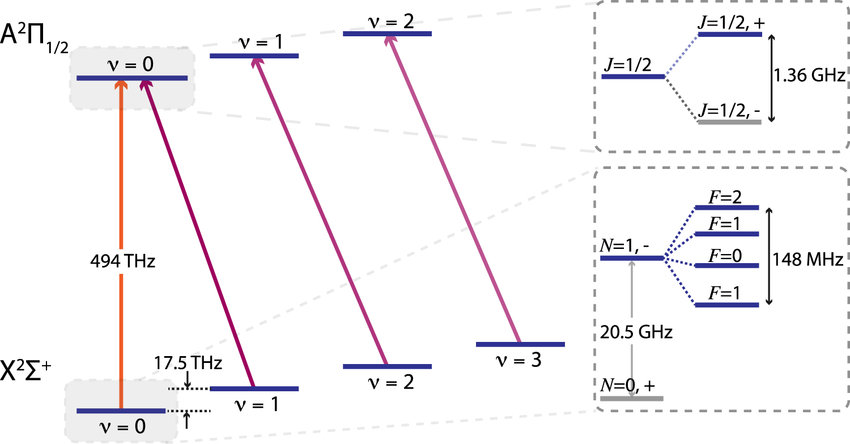
\includegraphics{img/Levels.png}
\end{center}

\paragraph*{Selection Rules}
Exitation subjected to $\Delta m = \pm 1$ for $\pi^\pm$ and $\Delta m = 0$ for $\sigma$.
Decay is arbitrary since the emission could have any polarization.
\par
Nuclear spin of \ce{F} is $1/2$ and \ce{Ca} is $0$.

\clearpage
\section{Script}

\paragraph*{Cover}
Today we are going to talk about this molecule Qubit.
The molecule is Calcium Monoflouride.
And they are able to create a Bell state in this system.


\paragraph*{Overview}
This is the overview of the experiment.
They use tweezers to move the molecules.
After initializing the qubits, they bring the molecules close to enable the electric dipole interaction, here.
This interaction turns out to give us a iSWAP gate.
And that's how they create entanglement.

\paragraph*{Outline}
We will first talk about the motivation, why we would like to use molecules.
And then we talk about how do they prepare the qubit.
The energy levels, and the initialization.
And then Mingkun will talk about further measurements and some outlook of this molecular manipulation.

\paragraph*{Motivation}

First is the motivation.
There is more complexities in the molecule.
Besides the electronic degrees of freedom, there is a vibrational motion and a rotational motion, and therefore we have two more quantum numbers and further split of electric energy levels.
And that's how the molecular energy levels differ from the atomic ones.

This molecule has a nonzero electric dipole interaction, which could be used to realize two-qubit operation.
Unlike in the Rydberg case, this dipole interaction is intrinsic / permanent.
This is because the dipole is due to the uneven charge distribution on two different nucleii.

And we will find that this qubit has a long coherence time.

\paragraph*{Qubit in CaF}
So here is the molecule.
The labels $X$ and $A$ denote electron energy levels.
$v$ is the vibrational energy level.
And $N$ is the rotation energy level.
The rest are similar to the atomic case.
One major different in molecular system is the selection rules.
In this case, the rotational level transition requires opposite parity.
The vibrational level transition is not quite restricted.
However, the transition probability are determined by the Frank-Condon factors.
If such factors are diagonal, then the transition of $v$ is not arbitrary.

We now apply these considerations to construct a closed optical transition.
We like closed optical transition because it limits our Hilbert space, and makes our manipulation easier.
So why this is closed?
The $N=0$ state has plus parity.
So the transition from $N=0$ to the excitation state is forbidden.
But the $N=1$ is allowed because they have opposite parity.
When the electron decays from the excitation state, it will fall back to the $N=1$ state, and with $v=0$ because the Frank-Condon factor is diagonal in this case.
{\color{red} Does it always fall back to $m_F=+2$ during the optical pumping initialization?}
This closed optical transition is related to the initialization process.

Then we select our qubits states.
They choose the up and down states here.
And the reason is to minimize the response to magnetic field and to minimize the AC stark shift.


\paragraph*{SPAM}
And then we go to the preparation.
We exploit the closed optical transition we just constructed.
They optically pump the $N=1$ manifold to the $\ket{D}$ state.
And then they do a microsweep from the $\ket{D}$ state to the $\ket{+}$ state and then to the $\ket{\uparrow}$ state.
And that's how they initialize their qubits to $\ket{\uparrow}$.
Then they remove the empty tweezers.
They use a kind of lambda-imaging to detect the molecules initialized to the $\ket{\uparrow}$ state.
And the rest are discarded.
The advantage of this approach is that they can do imaging while cooling down the motion.

And last is how they do qubit rotation.
They use a microwave drive to do a global rotation.


\par
{\color{red}What do they do to the $N=0$ states? Are they discarded at the QND step as unoccupied tweezers? Do the unoccupied tweezers refer to really unoccupied i.e. no molecule or refer to non $\ket{\uparrow}$ states? How do they tell apart $N=0$ and $\ket{+}$ as they claim $\ket{+}$ contributes 1\% of error?}

\clearpage

Circular ryd atoms: life close to seconds ($l=n-1$).



\paragraph*{Qubit in CaF}
Reason for close optical trans: limit our hilbert space, manipulation easier.
(Rotational) Parity limit $N=1$ to $A$.
Vib diagonal FC factors limit $v\rightarrow 0$.
Therefore, close op trans $X(N=1)\rightarrow A$.

Why choose this up down: insensitive to magnetic field and stark field. 
AC stark shift to zero (magic angle trap: apply mag field and polarization at certain angle).


\paragraph*{SPAM}
Init: close optical trans: optical pump to $\ket{D}$ state. Then microsweep to $\ket{\uparrow}$.


Detection: lambda-imaging.
Only detect up: how?
Lower level has no transition with $A$ state.
Non-destructive: why?



Advantage: imaging while cooling (motional state).
(Why not heat up mole while lambda imaging: because lambda imaging is related to lambda cooling ie when mole has nonzero veloci it absorb photon and (emit floureience) be kicked off and cool down. i.e. when it absorb a photon it cools down a little bit.)





Single qubit rotation: global single qubit rotation N.B. global micro wave, no single operation.



\paragraph*{Error in SPAM}

Overall fidelity 82 percent.
Reason:
\begin{itemize}
    \item Optical pumping nonperfect.
\end{itemize}


\paragraph*{Question}
\begin{itemize}
    \item SPAM fidelity: are all $N=0$ states thrown?
\end{itemize}

% \bibliographystyle{plain}
% \bibliography{main}

\end{document}
